\documentclass{beamer}
\usepackage[T1]{fontenc}
\usepackage[utf8]{inputenc}
\usetheme[secheader]{Boadilla}
\useinnertheme{rectangles}
\usepackage{helvet}
\definecolor{ecolol}{RGB}{156,201,14}
\setbeamercolor{alerted text}{fg=ecolol!80!white}
\setbeamercolor*{palette primary}{fg=ecolol!60!black,bg=white!85!ecolol}
\setbeamercolor*{palette secondary}{fg=ecolol!70!black,bg=white!60!ecolol}
\setbeamercolor*{palette tertiary}{bg=ecolol!80!black,fg=white!50!ecolol}
\setbeamercolor*{palette quaternary}{fg=ecolol,bg=white!20!ecolol}
\setbeamercolor*{sidebar}{fg=ecolol,bg=ecolol!75!white}
\setbeamercolor*{palette sidebar primary}{fg=ecolol!10!black}
\setbeamercolor*{palette sidebar secondary}{fg=white}
\setbeamercolor*{palette sidebar tertiary}{fg=ecolol!50!black}
\setbeamercolor*{palette sidebar quaternary}{fg=white!10!ecolol}
\setbeamercolor*{titlelike}{parent=palette primary}
\setbeamercolor{frametitle}{bg=white!90!ecolol}
\setbeamercolor{frametitle right}{bg=white!60!ecolol}
\setbeamercolor*{separation line}{}
\setbeamercolor*{fine separation line}{}
\setbeamercolor{block body}{parent=normal text,use=block title,bg=red!0,fg=}
\usepackage{eurosym}
\title{ELASTICSEARCH}
\subtitle{Search and analytics engine}
\date{26 mai 2016}
\author[]{WEEZHARD}
%Commentaire
\begin{document}
\begin{frame}
\titlepage
\end{frame}
\begin{frame}
\tableofcontents
\end{frame}
\section{Section ELK}
% \subsection{Contexte}
\begin{frame}
\frametitle{Stack ELK}
\begin{itemize}
\item  Logstash : Manifold for centralized logging , enrichment log and analysis.
\item  ElasticSearch : Data structure : distributed , scalable and highly available for research and data analysis.
\item  Redis : Memory data structure used as Broker for logs.
\item  Kibana : Web interface for data visualization ( charts, tables ) based on time.
\end{itemize}
\end{frame}
%
\begin{frame}
\frametitle{ELK : version of components}
\begin{itemize}
\item  Logstash : 2.3.2
\item  Elasticsearch : 2.3.3
\item  Redis : 3.0.6
\item  Kibana : 4.5.1
\end{itemize}
\end{frame}
%
\begin{frame}
\frametitle{ELK architecture}
\centering
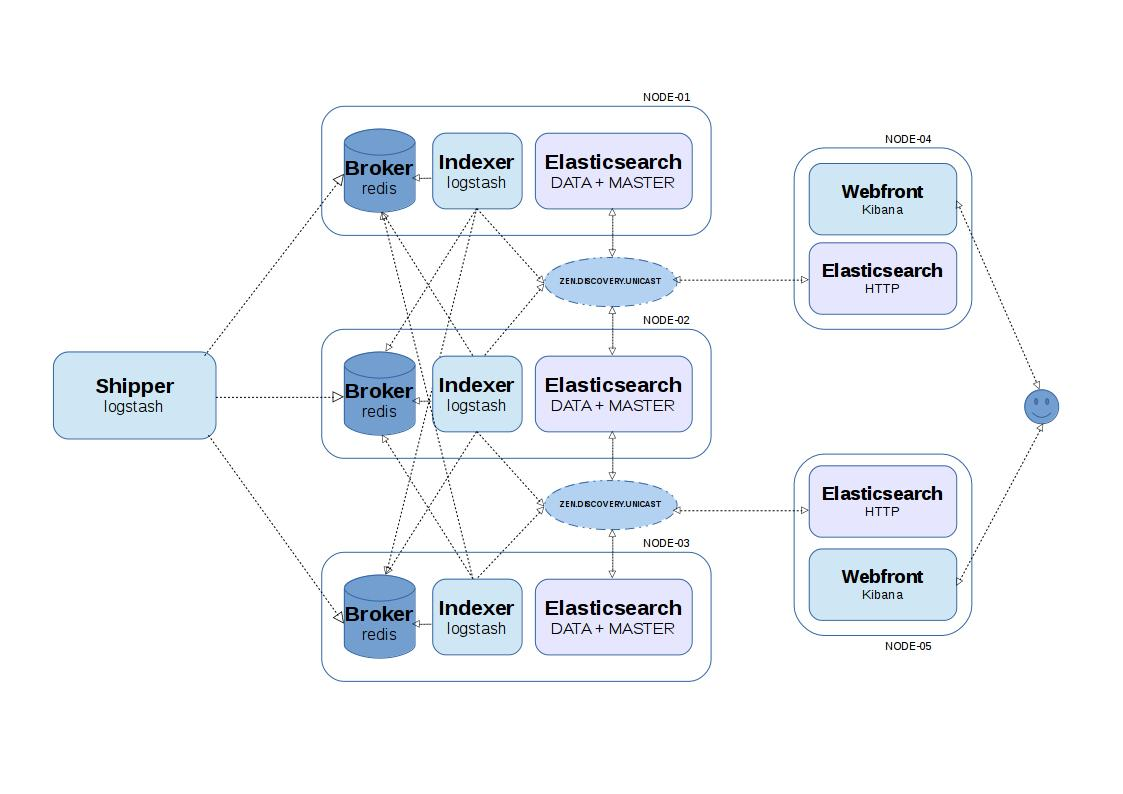
\includegraphics[scale=0.30]{img/elk_arch.jpg}
\end{frame}
%
\begin{frame}
\frametitle{ElasticSearch : Shard Placement Control}
\centering
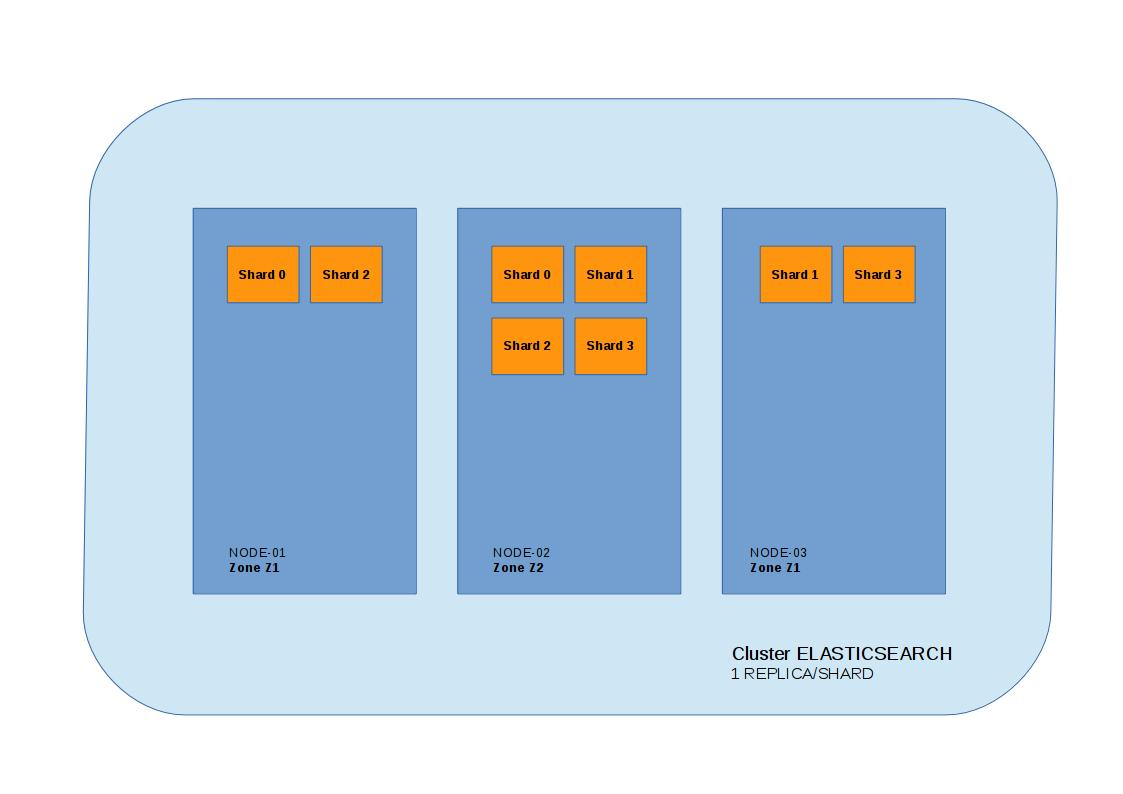
\includegraphics[scale=0.28]{img/elk_zone.jpg}
\end{frame}
%
\section{Section KIBANA}
% 
\begin{frame}
\frametitle{News (kibana 4)}
\begin{itemize}
\item The views : Discover, Visualize and dashboards are now independent.
\item A chart can be shared between multiple dashboards.
\item The interface is responsive
\item Plugin support : timelion, sense ...
\item Adding map geolocation.
\end{itemize}
\end{frame}
%
\begin{frame}
\frametitle{Modes}
\begin{itemize}
\item Discover: allows you to view data ElasticSearch index.
\item Visualize: allows to aggregate data into views .
\item Dashboard: allows you to build custom dashboards.
\end{itemize}
\end{frame}
\end{document}
